\documentclass[12pt]{scrartcl}

\usepackage[sorting=ynt,style=numeric]{biblatex}
\addbibresource{sources.bib}

\usepackage{graphicx}
\graphicspath{ {./images/} }

\usepackage{pdflscape}
\usepackage{tablefootnote}

\def\code#1{\texttt{\frenchspacing#1}}

\usepackage{hyperref}
\usepackage[htt]{hyphenat}

% \parskip=6pt
\usepackage[letterpaper,margin=1.25in]{geometry}
% \usepackage{parskip}

\usepackage{pgfplots, pgfplotstable}
\pgfplotsset{compat=1.15}
\pgfplotstableread[col sep=comma,]{data.csv}\datatable

% \let\oldsection\section
% \renewcommand\section{\clearpage\oldsection}

\begin{document}
\pagenumbering{roman}

\begin{titlepage}
    \begin{center}
        \vspace*{\fill}

        \Huge
        \textbf{TypeScript}

        \LARGE
        Final Report

        \vspace{0.5cm}
        \large
        Practical Course:\par
        Contributing to an Open-Source Project

        \vspace{5cm}

        Jonas Hübotter

        \small
        jonas.huebotter@tum.de

        \vspace{0.5cm}

        Technical University Munich

        March 16, 2021

        \vspace*{\fill}
    \end{center}
\end{titlepage}

% \section{Abstract}

\setcounter{tocdepth}{2}
\tableofcontents{}
\clearpage

\section{Introduction}
\pagenumbering{arabic}

TypeScript\footnote{\href{https://www.typescriptlang.org/}{TypeScript website}} is a programming language that extends JavaScript by adding types. It is funded by Microsoft and primarily developed by a dedicated team of Microsoft engineers. TypeScript is one of Microsoft's first ventures into open-source. Development on TypeScript began privately at Microsoft in 2010 \cite{Tung2020}. With the first release in 2012, TypeScript was made available freely under the Apache-2.0 License\footnote{\href{https://github.com/microsoft/TypeScript/blob/master/LICENSE.txt}{TypeScript license}}. First, the code was hosted on Microsoft's own forge website CodePlex before being moved to GitHub in 2014 \cite{Turner2014}. New feature releases of TypeScript are published every other month \cite{Rosenwasser2017}.

Today, the TypeScript GitHub repository\footnote{\href{https://github.com/Microsoft/TypeScript}{TypeScript repository}} has more than 69 thousand stars making it the 20th most starred repository on GitHub \cite{RepositoriesRanking}. The \code{typescript} package on NPM has over 19 million weekly downloads \cite{Package}. With more than 21 thousand dependent packages, TypeScript is the 24th most depended-upon package on NPM \cite{PackageDependents}. According to GitHub, almost 3.2 million public repositories depend on GitHub \cite{NetworkDependents}.

TypeScript's genesis was the surge in JavaScript development in the late 2000s as JavaScript runtimes became more efficient. With the rise of single page applications and Node.js supporting large JavaScript backends, the development and maintenance of large-scale JavaScript projects became a challenge \cite{Foley2012a}. Soma Somasegar, then Corporate Vice President of Microsoft’s Developer Division, summarized in 2012 that "we’re starting to see applications of unprecedented size written with JavaScript, despite the fact that creating large-scale JavaScript applications is hard. TypeScript makes it easier" \cite{Foley2012}. Anders Hejlsberg, one of TypeScript's lead developers, argued that refactoring becomes practically impossible using a programming language without static types and strong static analysis \cite{Cassel2019}.

The TypeScript project has particular significance as it marks a turning point in Microsoft's attitude towards open-source. The former CEO of Microsoft Steve Ballmer famously compared copyleft licenses to a "cancer that attaches itself in an intellectual property sense to everything it touches" \cite{ThomasCGreene2001} and also complained about a lack of accountability in open-source software \cite{JoeMcKendrick2003}. However, In recent years with the success of TypeScript and other open-source efforts at Microsoft this attitude has changed. Today, the company is the single biggest contributor to open-source in the world \cite{TomWarren2020}. According to Hejlsberg, the team developing TypeScript at Microsoft knew that they were only "going to appeal to the JavaScript community ... by being open source", but also noted that at the time Microsoft was ”very ambivalent” about open-source and even ”afraid” of it \cite{Tung2020}.

In this report, I critically reflect on my contributions and my communication with members of the TypeScript team as well as external contributors. Then, I examine systemic features of the development process on an individual and a project level. The report ends with suggestions towards increasing accessibility and engagement to further grow community support and contributions.

\section{Contributions}

This section gives a brief overview of all of my contributions to TypeScript. My contributions can largely be divided into three categories: contributions towards \textit{more accurate and concise error reporting}, contributions towards \textit{increased type safety} by strengthening existing or adding new type checks, and lastly contributions towards \textit{better type inference}. During the practical course I used a project board to track my work \cite{ProjectBoard}.

\subsection{Error reporting}

\begin{itemize}
    \item I worked on an improvement that reduced the length of the error message when a type is not assignable to a type parameter \cite{42849,42952}.
    \item I also worked on an improvement to make the error message more specific when the \code{typeof} operator should be omitted \cite{42523}. I published a pull request that implemented the improvement less than a day after the original issue was created and opened to external contributors \cite{42530}. Ultimately, we decided not to merge my changes as the creator of the original issue, Daniel Rosenwasser, realized that there was already another ongoing effort that prevented this error in the first place \cite{42530Comment}.
\end{itemize}

\subsection{Type safety}

\begin{itemize}
    \item The very first issue I worked on was an improvement to the type checks for the \code{in} operator\footnote{\href{https://developer.mozilla.org/en-US/docs/Web/JavaScript/Reference/Operators/in}{\code{in} operator}} \cite{41317}. Because it was a breaking change of type checks on a relatively common operator, quite a few design decisions had to be made \cite{41928}. My work and the conversations with the TypeScript team are discussed in greater detail as part of the case study in Section \ref{case_study}.
    \item I worked on an improvement that expanded the checks for uncalled functions to all operands of disjunctions \cite{35584,42835}. Previously only the rightmost argument of a disjunction was checked.
    \item Initially, my pull request mentioned in the previous point also expanded uncalled function checks to negations. Following the request of a reviewer \cite{42835Comment}, I extracted this improvement into a separate issue \cite{43096} and pull request \cite{43097}.
\end{itemize}

\subsection{Type inference}

\begin{itemize}
    \item When indexing the intersection type where one member is a tuple with an index that exceeded the length of that tuple, the resulting type is expected to be \code{undefined}. I fixed a bug that led the resulting type of such an indexing operation to be the union over all members of the tuple type, effectively treating the tuple as an infinitely long array \cite{42557,42602}.
    \item I also worked on a larger undertaking that improved the type inference for generic mapped types\footnote{\href{https://www.typescriptlang.org/docs/handbook/2/mapped-types.html}{Mapped Types}} \cite{37670,42382}. Nathan Fenner, an external contributor, supported this effort by reviewing my pull request and suggesting changes \cite{42382Comment}.
\end{itemize}

\subsection{Other work}

\begin{itemize}
    \item While first familiarizing myself with TypeScript's development environment I noticed that the documentation on inspecting changes to the test baselines in the contributing guidelines was outdated \cite{ContributingGuidelines}. I therefore created an issue and a pull request to update them \cite{41991,42031}.
    \item I also worked on an issue improving the specificity of the event type of the \code{readystatechange} event \cite{41775}. While working on this improvement I realized that even though the original issue was tracked in the TypeScript repository, the change had to be made in the \code{TypeScript-DOM-lib-generator} repository\footnote{\href{https://github.com/microsoft/TypeScript-DOM-lib-generator}{\code{TypeScript-DOM-lib-generator} repository}} as this is where the DOM types are specified. My pull request did not end up being merged due to a design decision trading performance for accuracy \cite{969Comment}.
\end{itemize}

\section{Communication}

I now discuss my communication with other contributors throughout the contributing process. To that end, I first debate general aspects of communication alongside specific examples. This is followed in Section \ref{quantitative_analysis} by a quantitative analysis of the iteration pace of my contributions.

The static documentation with which I refer to public documents like the contribution guidelines is very concise and up-to-date. I only found one passage on comparing test baselines that could be improved \cite{41991}. Likewise, the direct communication was always concise, inclusive, and either friendly or neutral. This was true regardless of whether communicating with external or internal contributors. I did not come across any violation of Microsoft's Code of Conduct that remained unaddressed\footnote{\href{https://opensource.microsoft.com/codeofconduct/}{Microsoft Code of Conduct}}.

Moreover, the direct communication always communicated intent clearly and efficiently. A good example of this is Daniel Rosenwasser's comment on my pull request which had to be closed as there was already another ongoing effort solving the issue:

\begin{quote}
    Thanks for the PR @jonhue! However, since I filed that issue yesterday, I've realized that maybe \#24738 is a better direction, where the type-checker will automatically promote well-known symbols to being unique. If we merge this in, we may have to back-out this change afterwards. \cite{42530Comment}
\end{quote}

Due to sometimes infrequent responses that are examined further in Section \ref{quantitative_analysis}, I occasionally considered reaching out privately to members of the TypeScript team. However, I ultimately decided to keep all communication public as in our meeting on creating a FLOSS project we came to the conclusion that in open-source projects public communication was generally preferable to private communication \cite{Priv1,13995Comment}.

\subsection{Quantitative analysis}
\label{quantitative_analysis}

In this section I give an overview of the \textit{iteration pace} of my contributions and show how certain features of issues and their related pull requests influence their iteration pace.

\subsubsection{Method}

In general, three features are used to differentiate between issues:

\begin{itemize}
    \item An issue is \textit{approved} once it was confirmed and labeled by a member of the TypeScript team. If it was labeled with \code{help wanted} external contributors may submit pull requests \cite{ContributingGuidelines}. At this stage issues are commonly also assigned to a milestone.
    \item An issue is \textit{scheduled} (or a milestone bug) once it was assigned to a milestone that is not the \code{Backlog} milestone. This may be an upcoming release of TypeScript, like in the case of the issue examined in Section \ref{case_study}.
    \item An issue is \textit{assigned} once it was assigned to a member of the TypeScript team. Commonly all scheduled issues are also assigned. Unscheduled issues are sometimes assigned too, but usually only after a pull request was opened.
\end{itemize}

In the following, I refer to these features as \textit{states}. Once a pull request is opened, a bot automatically shares the states of the issue addressed by the pull request with the pull request. We can therefore extend these issue states to their related pull requests.

The main quantities that are examined are the time between meaningful actions (\textit{response time}) and the percentage of meaningful actions that were at all responded to (\textit{response rate}). The \textit{absolute response rate} refers to the percentage of threads (issues and pull requests) where all actions have been responded to. Time differences are measured in days. A \textit{meaningful action} could be either a group of messages, a review, or updating some feature of the pull request like adding a label or moving the pull request within a project board\footnote{\href{https://github.com/jonhue/osp/tree/sources/analysis}{The complete list of meaningful actions}}. Further, meaningful actions are divided into \textit{immediate} responses to an action of the pull requests author and remaining responses.

\subsubsection{Results}

\begin{figure}
    \centering
    \begin{tikzpicture}
    \begin{axis}[width=15cm,
        height=10cm,
        ybar,
        bar width=0.5cm,
        ylabel={days},
        xtick=data,
        xticklabels from table={\datatable}{A},
        ymajorgrids]
        \addplot table [x expr=\coordindex, y=B]{\datatable};
        \addplot table [x expr=\coordindex, y=C]{\datatable};
        \addplot table [x expr=\coordindex, y=D]{\datatable};
        \legend{$\top$, $I$, $\neg I$}
    \end{axis}
    \end{tikzpicture}
    \caption{Average response time by state \\ ($\top \sim$ any, $S \sim$ scheduled, $A \sim$ assigned, $I \sim$ immediate)}
    \label{fig:response_time_states}
\end{figure}

The average response time among all $40$ analyzed responses was $4.9$ days and is shown in Figure \ref{fig:response_time_states}. $8$ responses of issues were analyzed with an average response time of $2.1$ days, whereas the remaining $32$ responses to pull requests had an average response time of $5.5$ days which was even higher when only counting the $29$ responses by the TypeScript team ($6$ days). Despite the small sample size, it can be concluded that there is a significant disparity in how fast the TypeScript team reacts to issues when compared to pull requests which is likely explained by an effort to prevent the build-up of a backlog of issues.

Further, it can be seen that there is no substantial difference in iteration pace between scheduled and assigned tickets with around $1.5$ days on average between responses. On the other hand, unscheduled and unassigned tickets perform significantly worse with an average response time of more than $7$ days and almost $9$ days for pull requests. So on average, the iteration pace of scheduled and assigned tickets is about $5$ times faster.

The average response time of the $28$ immediate responses ($5$ days) is slightly higher than the average response time of the remaining responses ($4.7$ days). A very interesting observation is, however, that for scheduled and assigned tickets the immediate responses ($0.6$ days and $1$ day, respectively) are faster than the average response ($1.4$ days and $1.6$ days, respectively). This reverses when considering unscheduled tickets where immediate responses on average take more than a day longer. Likewise, for unassigned tickets immediate responses take longer on average than other responses.

One attempt at explaining this asymmetry leads to the following insight: The non-immediate responses are influenced less by the ticket status than immediate responses as they have a higher dependency on internal development processes of the TypeScript team. Once a team member is assigned to a ticket or a ticket was scheduled, there appears to be a considerably higher perceived responsibility incentivizing quicker responses. Whereas, for unscheduled and unassigned tickets, once they are close to being merged, the internal processes do not take as much longer as the reduced perceived responsibility increases the immediate response time.

The average response rate of the $16$ examined threads was $81\%$ while the absolute response rate was $63\%$. On average, the response rate was slightly higher in pull requests than in issues ($83\%$ compared to $78\%$). On the other hand, the absolute response rate was higher in issues than in pull requests ($71\%$ compared to $56\%$). This discrepancy can be explained with the higher number of overall actions in pull requests that diminish the effect of single actions that were not responded to.

The average time until a pull request was closed was $30.4$ days assuming open pull were closed at the 16th of March 2021. Of the $9$ pull requests considered, $4$ were closed. On average, my pull requests received $9.8$ comments. Totaling $44$ comments, the longest conversation evolved around strengthening type checks for the \code{in} operator \cite{41317} which is discussed in the following section \ref{case_study}.

\section{Case study}
\label{case_study}

In this case study I examine the work process and communication with the TypeScript team as exemplified by my work on improving the type checks for the \code{in} operator \cite{41317}. I begin by describing the TypeScript development environment which is an essential part of the contribution process. Then, I discuss specific aspects of this particular contribution and how my approach generalized to other contributions. This is followed by an examination of the iteration process where I debate the communication as part of the pull request and the design decisions that were made along the way. Finally, I summarize how this contribution related to my other contributions.

\subsection{Development environment}

TypeScript is bootstrapped, that is TypeScript itself is written in TypeScript. Therefore, cloning, setting up development tools, and installing dependencies is fast and well-documented \cite{ContributingGuidelines}. There are two main aspects of the development environment that I examine: the development environment when working on the source files of TypeScript and when writing tests.

The core of the TypeScript compiler is implemented in relatively few files in \break\code{src/compiler}. The fundamental parts like scanning, parsing, type-checking, and code generation largely live in single isolated files. Therefore, these files are rather large. The type-checking and type-inference algorithm which was the subject of most of my contributions, is implemented in \code{checker.ts} which spans more than 41 thousand lines of code \cite{CheckerFile}. This comes with some drawbacks that are discussed further in Section \ref{feedback}. One immediate consequence is, however, that regardless of which particular editor is used, running static analysis on an edited file is very slow.

The tests can be divided into two categories. There are automated tests that are run on every single commit and are part of the TypeScript repository \cite{ContributingGuidelines} and there are user tests that run on actual TypeScript implementations. These latter tests are invoked by members of the TypeScript team on pull requests as needed and run by a bot \cite{UserTests}.

A test case is a single TypeScript source file. When a test case is run, TypeScript generates multiple files including the generated JavaScript, the inferred type of every expression, and the errors produced by the compiler \cite{ContributingGuidelines}. These files are tracked by Git under \code{tests/baselines/reference} and also referred to as baselines. A local test run produces updated baselines in \code{tests/baselines/local} which can then be compared to the tracked baselines and accepted if the differences are valid \cite{ContributingGuidelines}. A launch config for VS Code is also provided which can be used to launch test cases directly from the editor \cite{ContributingGuidelines}. Possible improvements to this test system are discussed in Section \ref{feedback}.

\subsection{Development process}
\label{development_process}

Now, I discuss specifics of the given issue and how I implemented a first solution in greater detail. The problem was to ensure that the right operand of the \code{in} operator is not a primitive type at runtime as the ECMAScript spec requires this operand to be an object \cite{InOperator}. If a primitive type is given, a runtime error is thrown. There are, however, a multitude of nuances between allowing any value as the right operand and absolute insurance that the right operand can never be a primitive. The problem was not to detect when the right operand was a primitive literal (like in the expression \code{key in 42}) as this was already detected by the compiler. The problem was to detect when a value was used as the right operand whose type \textit{could} potentially be a primitive, for example because its type was an unconstrained type parameter.

This specific issue already had an ongoing conversation where Andrew Branch, the TypeScript team member who was assigned to the issue, already indicated which function a potential fix would need to change \cite{41317Comment}. This was incredibly helpful. For other issues, the main difficulty was to determine \textit{where} a change should go rather than \textit{what} the change should be. The process that worked best in most cases was to start with a test case that reproduced the problem by throwing an error (all problems affecting type inference or type checking can be specified in such a way), to identify where this error is added in the type checker and then use call traces to determine where the change has to be made. Naturally, this approach works better with type checking problems where the problematic area is \textit{closer} to the place where the error is added. For type inference problems where the problematic area may be very far away from this place, this approach is less ideal.

Once I determined the problematic area, I made changes until the reproducible test case was behaving as expected. Then I ran the code on an increasingly larger number of tests. I quickly realized how delicate the behavior of the type inference and type checking code is. Because it is very interrelated and there are usually many different contexts in which some piece of code is run, even a very small change can have a tremendous impact on the behavior of the compiler. For example, when I restricted the type of the right operand of the \code{in} operator too much, there were many test cases failing even if they had not been explicitly testing type checking of the \code{in} operator (TODO: cite).

\subsection{Iteration on the public pull request}

The here examined issue was already assigned to a member of the TypeScript team, namely Andrew Branch, and scheduled for the 4.2 release of TypeScript \cite{41317}. As was shown in Section \ref{quantitative_analysis}, this issue could already be expected to receive more traction than others.

\begin{figure}
    \centering
    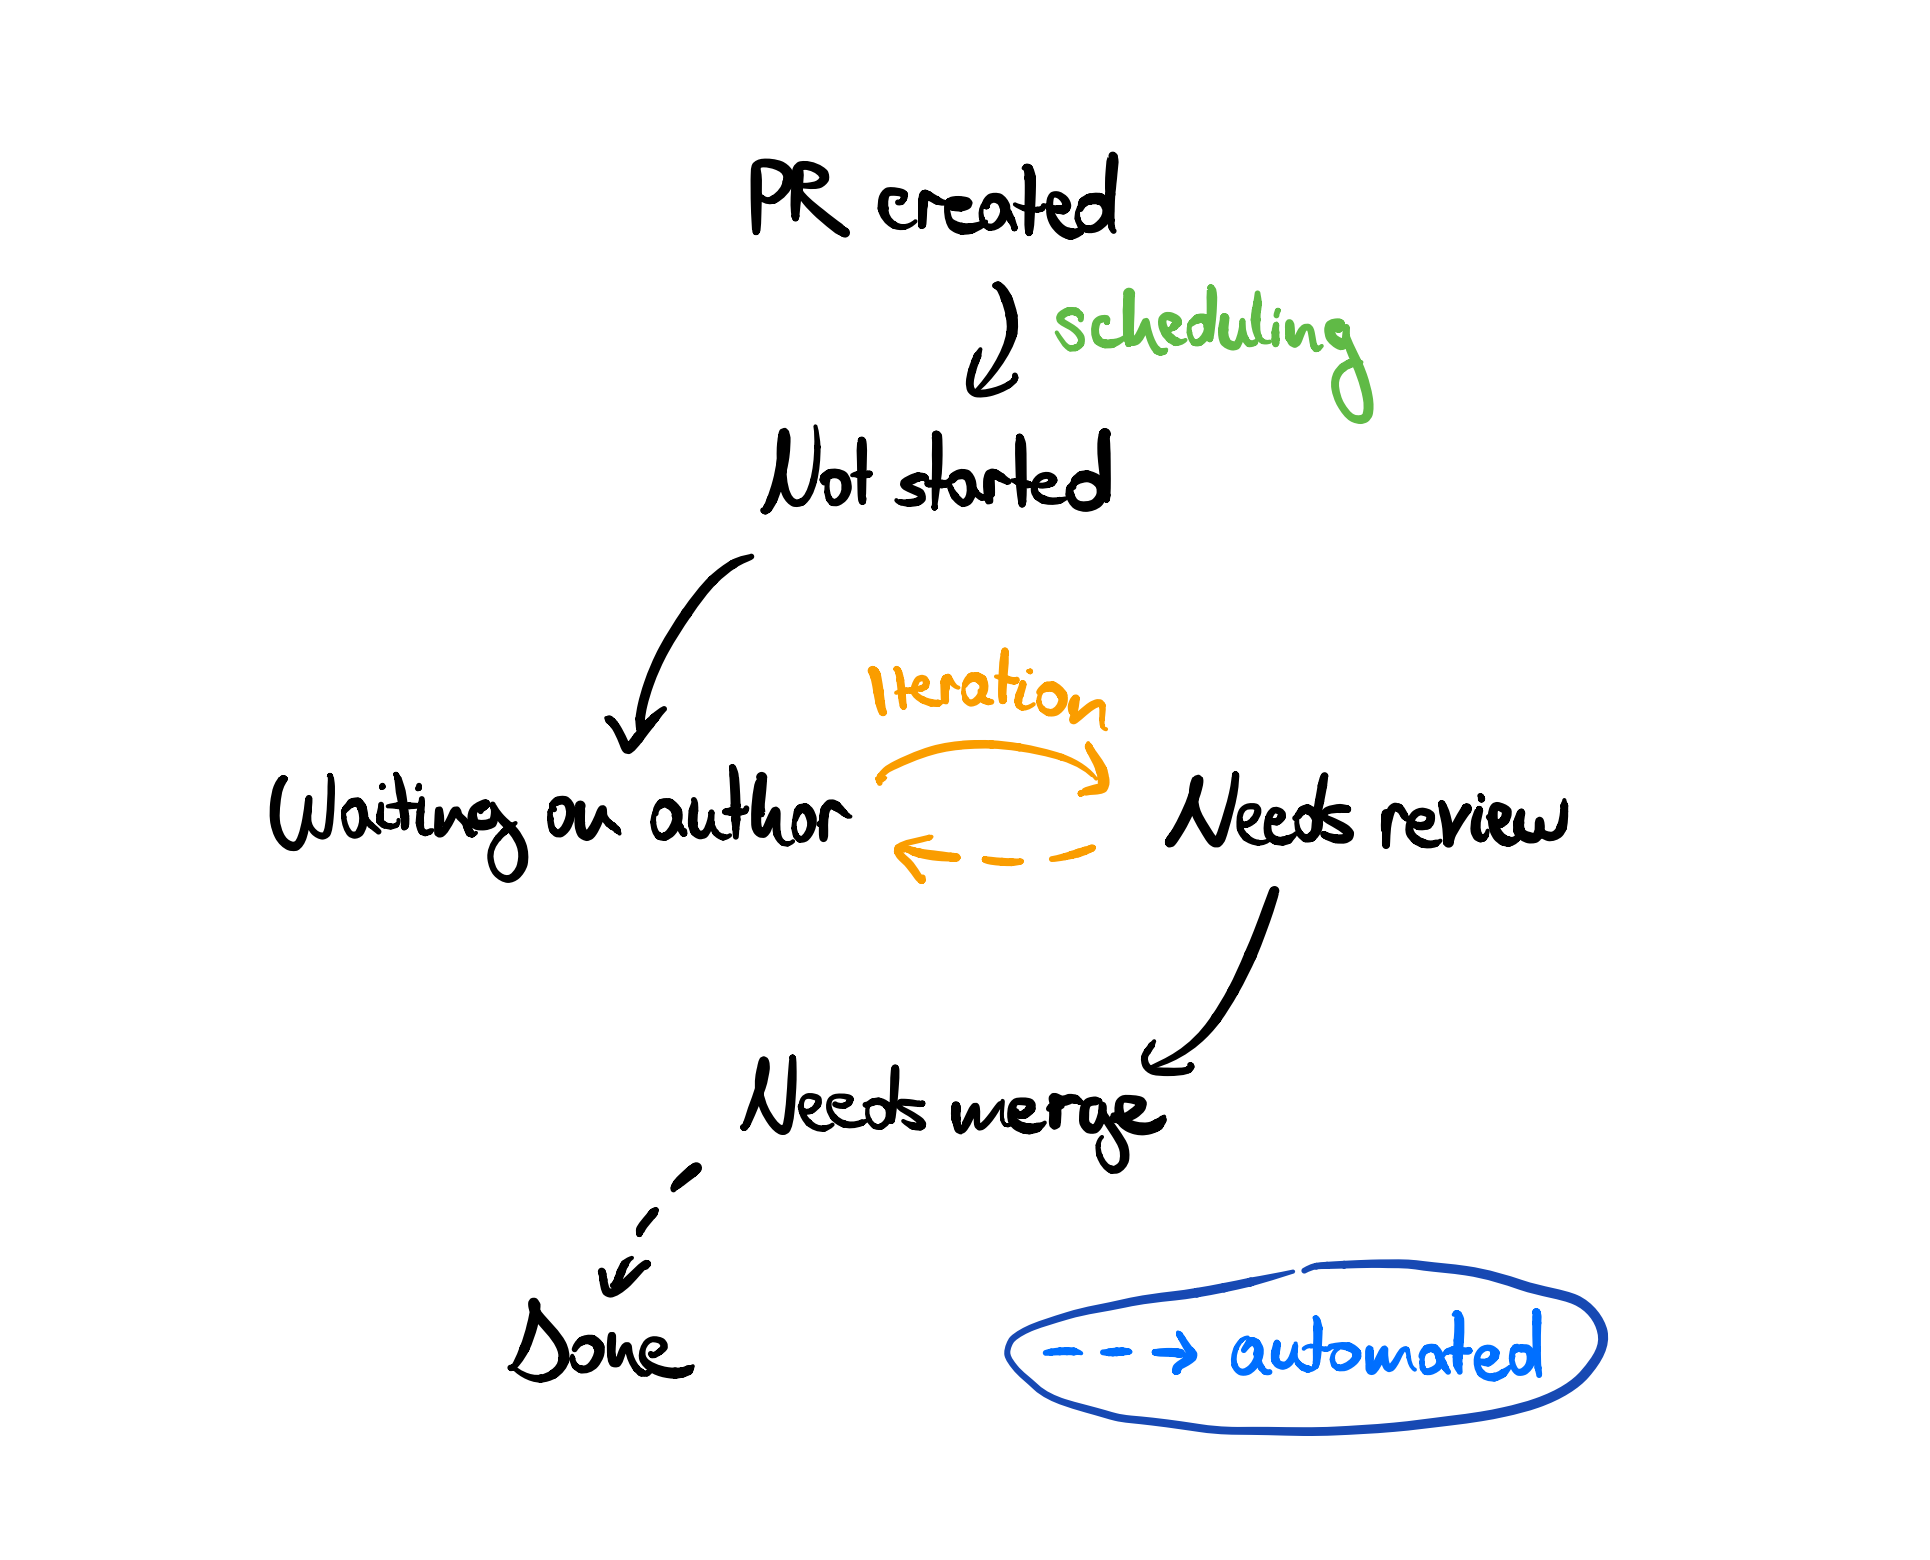
\includegraphics[width=10cm]{images/pr_backlog.png}
    \caption{PR Backlog process}
    \label{fig:pr_backlog}
\end{figure}

The TypeScript team tracks reviews of pull requests with a dedicated \code{PR Backlog} project board on GitHub \cite{PRBacklog} illustrated in Figure \ref{fig:pr_backlog}. New pull requests are manually added to \code{Not started}. During the iteration process, pull requests cycle between \code{Waiting on author} and \code{Needs review}. Once a pull request is close to a merge, it is moved to \code{Needs merge} from where it is automatically moved to \code{Done} once it was merged.

During the iteration process of the examined issue \cite{41928}, mainly two design decisions had to be made. Namely, we had to find an accurate and concise error message and tune the strictness of the type check. The latter, in particular, required multiple rounds of iteration. This was because we had to strike a balance between type safety and breaking as little code as possible. My initial solution worked by ensuring the right operand of an \code{in} expression was not assignable to a primitive type like \code{number} or \code{string} \cite{41928Comment1}. Due to a limitation with narrowing type parameters \cite{13995} that would have made it difficult to enforce these stronger type checks in practice,. Therefore, a more conservative fix was suggested by members of the TypeScript team that only ensures that the resolved constraint of the right operand's type is not assignable to a primitive \cite{41928Comment2}. These solutions sound similar at first, however, the latter is a negative check ensuring that the type of the right operand does not explicitly extend a primitive type while the former solution is a positive check that the type of the right expression cannot possibly extend a primitive type. Ultimately, the decision to opt for weaker type safety reaffirms TypeScript's focus on usability and unobtrusiveness \cite{RyanDonovan2020}.

This exemplified by a comment by Ryan Cavanaugh, the lead developer of TypeScript, on the expression \code{typeof val === 'object' \&\& '\_\_isMaybe' in val} which lead to an error with my initial implementation:

\begin{quote}
    This error is \textit{actually correct} --- \code{val} could be \code{null} --- but boy are we going to get bug reports about this. Maybe we need to special-case the error message. \cite{41928Comment3}
\end{quote}

Because this was such a wide-ranging change, in some additional rounds of iteration test coverage had to be widened \cite{41928Comment4}. While opening the pull request, I forgot to allow maintainers to edit my branch. As a consequence, my pull request was closed immediately before being merged so that Andrew Branch could make a few final changes to the error message \cite{42288}.

\subsection{Summary and comparison to other contributions}

The work on this issue has been very enjoyable. The conversation was always friendly, comments were concise, and intentions were communicated clearly. It was of tremendous help that the reviewers included examples in their comments like when Andrew Branch was suggesting to widen the test coverage \cite{41928Comment4}.

Most importantly, however, the iterations were fast paced. This gave everyone a sense that this issue was moving in the right direction. This is exemplified by an average \textit{immediate response time} of $0.7$ days compared to an average immediate response time across all contributions of $5$ day. Also, the \textit{response rate} was $100\%$ compared to an overall response rate to pull requests of $83\%$ (Section \ref{quantitative_analysis}).

\section{Feedback and suggestions}
\label{feedback}

A well-documented and precise contribution process is perhaps the most important feature of an open-source repository with regards to reducing friction for contributors. This already works very well within the TypeScript project. One specific feature of how contributions are handled is that incoming issues are processed rapidly and labeled accurately with one of 127 labels. If an issue does not meet the criteria outlined in the contribution guidelines or will not be worked on, it is closed quickly. This policy is very effective in reducing noise. Additionally, the number of labels and their active usage make issues and pull requests very searchable. All of the above means in practice that one rarely finds an issue that is not still prevalent and it is easy to restrict searches to a very narrow domain of interest. Further, by requiring the use of the TypeScript playground\footnote{\href{https://www.typescriptlang.org/play}{TypeScript playground}}, it is incredibly easy for contributors to reproduce issues and determine in which versions they are prevalent.

Anders Hejlsberg claimed in an interview in 2020 that since its move to GitHub in 2014, TypeScript has not only been open-source but also doing their "entire development process in the open" \cite{Tung2020}. While it is true that most conversations around the development of tracked issues are open, feature-planning is still done privately by the TypeScript team. Opening this process, for example by allowing the community to vote on new features, would almost certainly increase community engagement. Additionally, as of now, almost all new features are implemented by the TypeScript team. Together with a more transparent tracking of planned features, opening the development of new features to the community, could further increase the excitement of contributors. In an interview last year, Ryan Cavanaugh acknowledged this:

\begin{quote}
    The main challenge we see there is that adding features to the TypeScript code base is actually easy and fixing bugs is really hard. People are a lot more excited to add features than fix bugs because it’s fun. Who can blame them? Figuring out what we can do about that and encouraging people to help us out on the things we need more help with would be a community challenge. \cite{RyanDonovan2020}
\end{quote}

Starting to work on a project as big as the TypeScript compiler might seem somewhat daunting for many potential contributors. This is where mentoring and a place to ask questions can help. In our conversation with Stephan Kulla on his experience with Serlo we learnt that onboarding people to a large project and continuously mentoring them increases their excitement about their work \cite{Priv2}. The TypeScript Discord\footnote{\href{https://discord.gg/typescript}{TypeScript Discord}} is offering precisely that, but it could be featured more prominently in the projects Readme and Contributing Guidelines.

As Ryan Cavanaugh also pointed out in the mentioned interview, "rather than growing the team, [they] just hope to grow the community to support TypeScript" \cite{RyanDonovan2020}. To support a growing community, however, it is essential that the processes are able to sustain a growing number of contributions without growing the team. With the discussed PR Backlog serving as an example \cite{PRBacklog}, the team already has such processes in place. As we saw in Section \ref{quantitative_analysis}, for some contributions interactivity is rather low. Increasing the iteration pace would definitely increase the happiness amongst contributors. To that end, one first potential step could be to automate more steps of the PR Backlog workflow by extending the already existing TypeScript bot to automatically move pull requests within the PR Backlog project once an author addressed review feedback.

Finally, to increase contributions, it is extremely important to lower the barrier to entry and to reduce friction during development. Especially for a large and arguably complicated project like TypeScript, increasing code quality is very important. In addition, a document that explains the purpose of each module would make it easier for first-time contributors to understand where to start. The biggest potential of making development easier lies with improving debugging and the performance of tests because (as discussed in Section \ref{development_process}) this is where most time is spent during development. Yet, especially the latter is difficult to improve. This is because TypeScript relies on a large number of behavioral tests to test for correct behavior. With each pull request and fixed issue a new behavioral test is added, but only very rarely tests are removed. As there is a potentially infinite number of behavioral tests, defining a strategy of how to limit test execution time would be beneficial. This might be achieved by better structuring tests to reduce duplication or by extracting some classes of rarely broken tests to be only run once before a merge.

\section{Conclusion}

Throughout the past months, I found it very enjoyable to work on TypeScript. I had many interesting conversations with both members of the TypeScript team and other external contributors. It was fascinating and extremely rewarding to work on features like type checking and type inference that are immensely interrelated and eventually see my contributions improve the static analysis of so many programs.

T sometimes infrequent conversations made precise communication even more important. I adapted and improved that aspect over the course of the past months. I also learnt that in almost all cases it is best to keep the scope of pull requests to an absolute minimum to reduce the number of iterations.

Over the last few years TypeScript exemplified Microsofts journey towards more open-source development. TypeScript has come very far from where it started when published in 2012, but its journey towards a more open development is not yet finished. In the coming years it will be important to further increase community participation. As one of the largest open-source projects with growing adoption and more and more people wanting to contribute, it also remains important to update development processes, to sustain that growth.

\clearpage

\printbibliography

\clearpage
\appendix

\begin{landscape}
\section{Pull request overview}
\begin{table}[!h]
\begin{tabular}{ l r r r r }
 Tag & Days until first review & Days until close & Comments & Number of participants\tablefootnote{excluding bots} \\\hline
 \href{https://github.com/microsoft/TypeScript/pull/43097}{\code{TypeScript\#43097}} & - & - & 0 & 1 \\
 \href{https://github.com/microsoft/TypeScript/pull/42835}{\code{TypeScript\#42835}} & 13 & - & 11 & 2 \\
 \href{https://github.com/microsoft/TypeScript/pull/42602}{\code{TypeScript\#42602}} & - & - & 3 & 2 \\
 \href{https://github.com/microsoft/TypeScript/pull/42382}{\code{TypeScript\#42382}} & 11 & - & 14 & 3 \\
 \href{https://github.com/microsoft/TypeScript/pull/42952}{\code{TypeScript\#42952}} & - & 9 & 1 & 2 \\
 \href{https://github.com/microsoft/TypeScript/pull/42530}{\code{TypeScript\#42530}} & 0 & 6 & 10 & 2 \\
 \href{https://github.com/microsoft/TypeScript-DOM-lib-generator/pull/969}{\code{TypeScript-DOM-lib-generator\#43097}} & 1 & - & 4 & 3 \\
 \href{https://github.com/microsoft/TypeScript/pull/42031}{\code{TypeScript\#42031}} & 1 & 17 & 1 & 4 \\
 \href{https://github.com/microsoft/TypeScript/pull/41928}{\code{TypeScript\#41928}} & 0 & 32 & 44 & 5
\end{tabular}
\end{table}
\end{landscape}

\end{document}
